\documentclass[8pt, A4]{article}    %twocolumn

\usepackage[utf8]{inputenc}
\usepackage[normalem]{ulem}   % Para tachar
\usepackage{verbatim}
\usepackage{lipsum}
\usepackage[spanish]{babel}
\usepackage[hidelinks]{hyperref}
\usepackage{color}
\usepackage[dvipsnames]{xcolor}
\usepackage{kantlipsum}
\usepackage{graphicx}
\usepackage[margin=2.5cm]{geometry}
\usepackage{import}
\usepackage{listings}
\usepackage{amsmath}

\newcommand\tab[1][1cm]{\hspace*{#1}}

\newcommand{\grisclaro}{\color[gray]{0.99}}
\newcommand{\gris}{\color[gray]{0.9}}
\newcommand{\grisos}{\color[gray]{0.5}}

\newcommand{\showprog}[1]
{
\begin{minipage}{\textwidth}
\lstinputlisting[language=C++,
                  frame=single,
		  backgroundcolor=\grisclaro,
		  extendedchars=false,
          inputencoding=utf8,
		  aboveskip=1eM,
		  belowskip=1.5eM,
		  basicstyle=\small,
		  title=-- #1 --,
		  xleftmargin=1cm,
		  xrightmargin=1cm,
		  columns=flexible,
		  keywordstyle=\color{blue}\ttfamily,
		stringstyle=\color{red}\ttfamily,
		  commentstyle=\color{green}\ttfamily]
 {code/#1}
\end{minipage} 
}

\newcommand { \bold }[1]{\textbf{#1}}

\title{Análisis de Algoritmos de Ordenación}
\author{Alberto Robles Enciso}
\date{Febrero de 2018}

\begin{document}


\maketitle

\begin{figure}[h]
\begin{center}
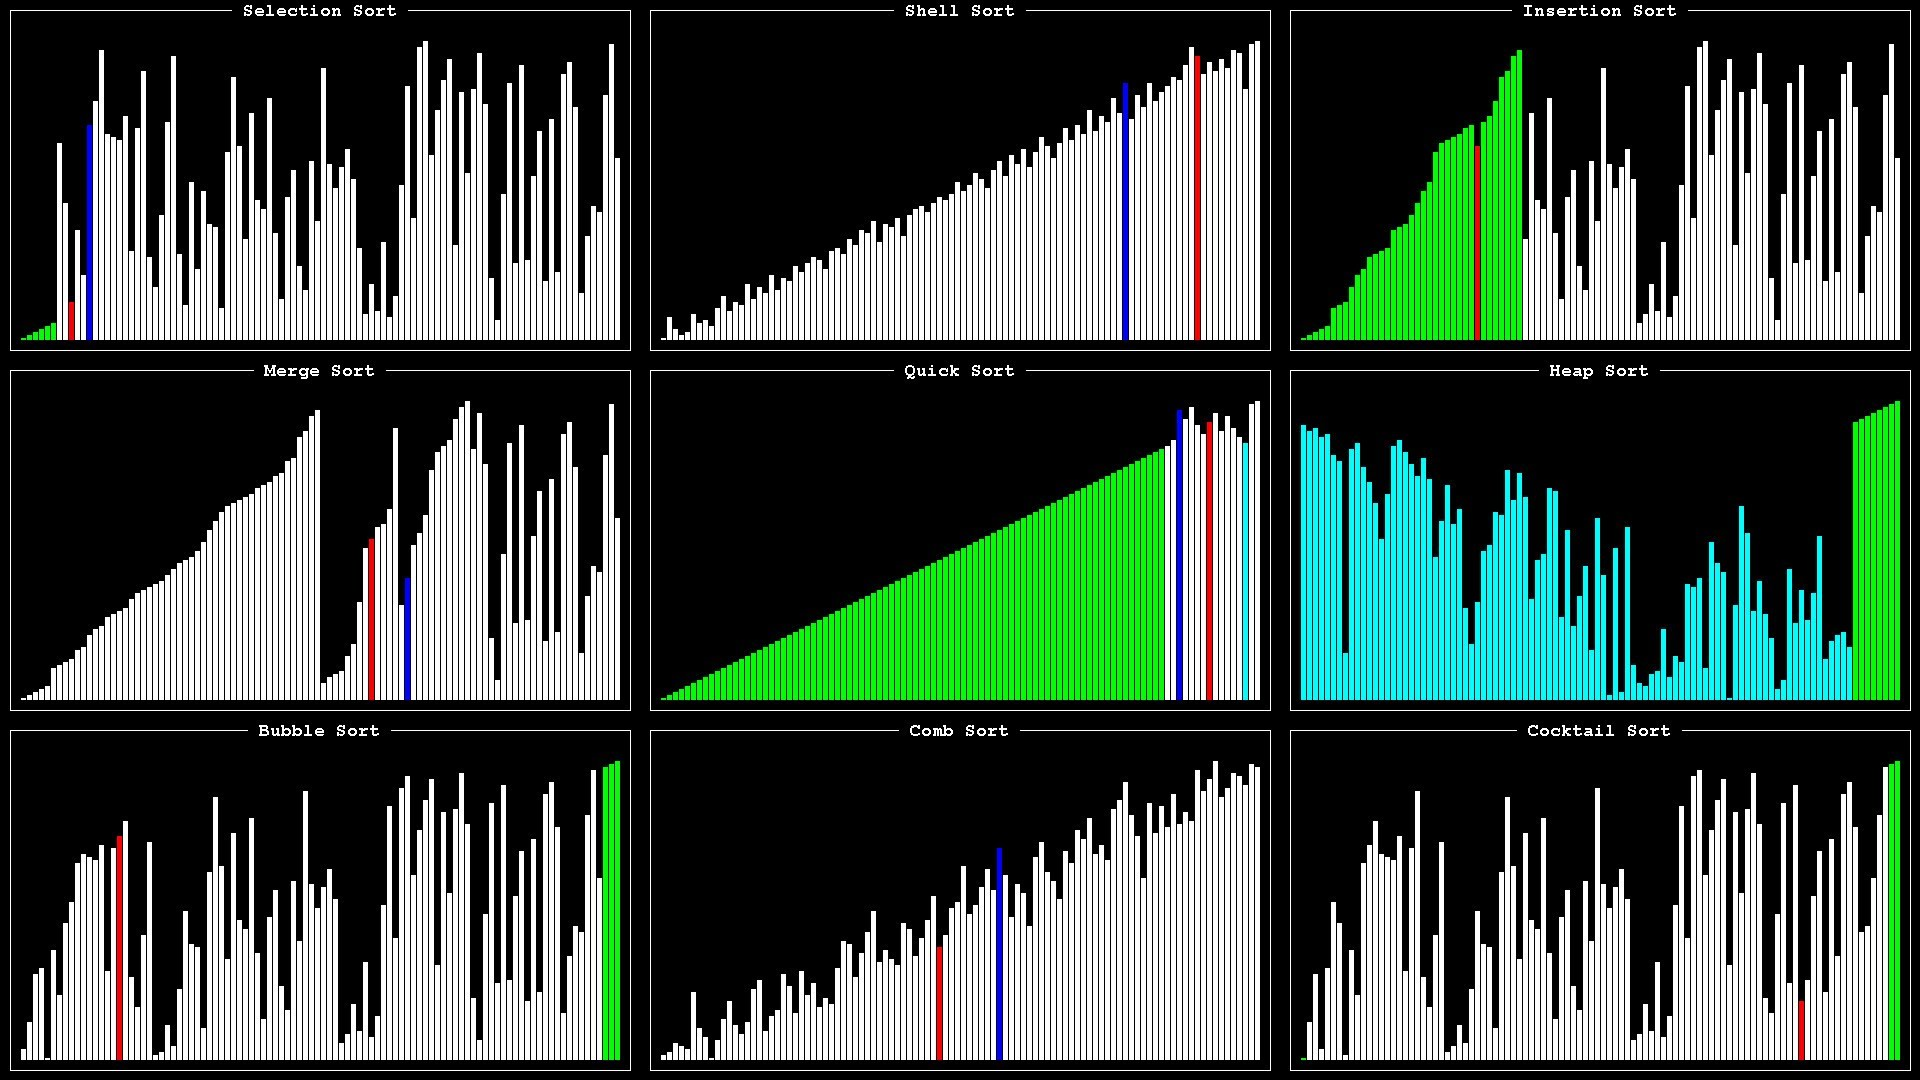
\includegraphics[width=1\textwidth]{graph/intro}
\end{center}
\end{figure}

\begin{abstract}
En este documento se va a analizar tres algoritmos de ordenación para determinar orden computacional teóricamente y experimentalmente.
\end{abstract}

\newpage

\tableofcontents

\newpage

\section{Introducción}
En computación y matemáticas un algoritmo de ordenamiento es un algoritmo que pone elementos de una lista o un vector en una secuencia dada por una relación de orden, es decir, el resultado de salida ha de ser una permutación —o reordenamiento— de la entrada que satisfaga la relación de orden dada. Las relaciones de orden más usadas son el orden numérico y el orden lexicográfico. Ordenamientos eficientes son importantes para optimizar el uso de otros algoritmos (como los de búsqueda y fusión) que requieren listas ordenadas para una ejecución rápida. También es útil para poner datos en forma canónica y para generar resultados legibles por humanos.

\section{Clasificación}
Los algoritmos de ordenamiento se pueden clasificar en las siguientes maneras:

\begin{itemize}
	\item La más común es clasificar según el lugar donde se realice la ordenación
	\begin{itemize}
		\item Algoritmos de ordenamiento interno: en la memoria del ordenador.
		\item Algoritmos de ordenamiento externo: en un lugar externo como un disco duro.
	\end{itemize}
	\item Por el tiempo que tardan en realizar la ordenación, dadas entradas ya ordenadas o inversamente ordenadas:
	\begin{itemize}
		\item Algoritmos de ordenación natural: Tarda lo mínimo posible cuando la entrada está ordenada.
		\item Algoritmos de ordenación no natural: Tarda lo mínimo posible cuando la entrada está inversamente ordenada.
	\end{itemize}
	\item Por estabilidad: un ordenamiento estable mantiene el orden relativo que tenían originalmente los elementos con claves iguales. Por ejemplo, si una lista ordenada por fecha se reordena en orden alfabético con un algoritmo estable, todos los elementos cuya clave alfabética sea la misma quedarán en orden de fecha. Otro caso sería cuando no interesan las mayúsculas y minúsculas, pero se quiere que si una clave aBC estaba antes que AbC, en el resultado ambas claves aparezcan juntas y en el orden original: aBC, AbC. Cuando los elementos son indistinguibles (porque cada elemento se ordena por la clave completa) la estabilidad no interesa. Los algoritmos de ordenamiento que no son estables se pueden implementar para que sí lo sean. Una manera de hacer esto es modificar artificialmente la clave de ordenamiento de modo que la posición original en la lista participe del ordenamiento en caso de coincidencia.
\end{itemize}

Los algoritmos se distinguen por las siguientes características:
\begin{itemize}
	\item Complejidad computacional (peor caso, caso promedio y mejor caso) en términos de n, el tamaño de la lista o arreglo. Para esto se usa el concepto de orden de una función y se usa la notación $O(n)$. El mejor comportamiento para ordenar (si no se aprovecha la estructura de las claves) es $O(nlog n)$. Los algoritmos más simples son cuadráticos, es decir $O(n^2)$. Los algoritmos que aprovechan la estructura de las claves de ordenamiento (p. ej. bucket sort) pueden ordenar en $O(kn)$ donde k es el tamaño del espacio de claves. Como dicho tamaño es conocido a priori, se puede decir que estos algoritmos tienen un desempeño lineal, es decir $O(n)$.
	\item Uso de memoria y otros recursos computacionales. También se usa la notación $O(n)$.
\end{itemize}

\newpage

\section{Algoritmos de Ordenacion}

\subsection{Ordenamiento de burbuja}
La Ordenación de burbuja (Bubble Sort en inglés) es un sencillo algoritmo de ordenamiento. Funciona revisando cada elemento de la lista que va a ser ordenada con el siguiente, intercambiándolos de posición si están en el orden equivocado. Es necesario revisar varias veces toda la lista hasta que no se necesiten más intercambios, lo cual significa que la lista está ordenada. Este algoritmo obtiene su nombre de la forma con la que suben por la lista los elementos durante los intercambios, como si fueran pequeñas "burbujas" (se puede ver un ejemplo de su funcionamiento en la figura \ref{fig:BubbleSortInfo}). También es conocido como el método del intercambio directo. Dado que solo usa comparaciones para operar elementos, se lo considera un algoritmo de comparación, siendo uno de los más sencillo de implementar.

\begin{figure}[h]
\begin{center}
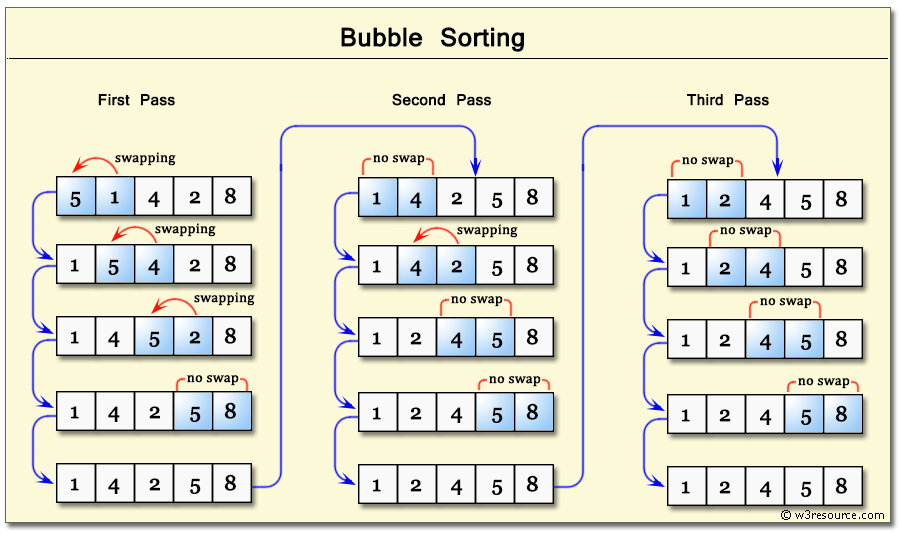
\includegraphics[width=1\textwidth]{graph/bubble-short-info}
\end{center}
\caption{Ejemplo de funcionamiento del algoritmo Bubble Short}
\label{fig:BubbleSortInfo}
\end{figure}

\subsubsection{Descripción}
Una manera simple de expresar el Bubble Sort en pseudocódigo es indicado en la figura \ref{fig:BubbleSortCode}.

\begin{figure}[h]
\begin{center}
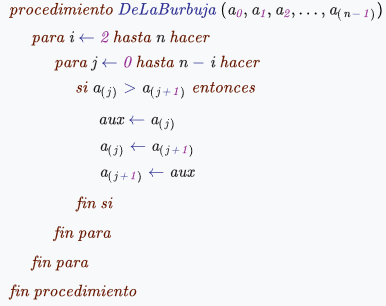
\includegraphics[width=0.5\textwidth]{graph/bubble-short-code}
\end{center}
\caption{Pseudocódigo del algoritmo Bubble Short}
\label{fig:BubbleSortCode}
\end{figure}

Este algoritmo realiza el ordenamiento o reordenamiento de una lista a de n valores, en este caso de n términos numerados del 0 al n-1; consta de dos bucles anidados, uno con el índice i, que da un tamaño menor al recorrido de la burbuja en sentido inverso de 2 a n, y un segundo bucle con el índice j, con un recorrido desde 0 hasta n-i, para cada iteración del primer bucle, que indica el lugar de la burbuja.

La burbuja son dos términos de la lista seguidos, j y j+1, que se comparan: si el primero es mayor que el segundo sus valores se intercambian.

Esta comparación se repite en el centro de los dos bucles, dando lugar a la postre a una lista ordenada. Puede verse que el número de repeticiones solo depende de n y no del orden de los términos, esto es, si pasamos al algoritmo una lista ya ordenada, realizará todas las comparaciones exactamente igual que para una lista no ordenada. Esta es una característica de este algoritmo. Luego veremos una variante que evita este inconveniente.

Para comprender el funcionamiento, veamos un ejemplo sencillo:

Tenemos una lista de números que hay que ordenar:

\tab ${\displaystyle a=\{55,86,48,16,82\}\,}$

Podemos ver que la lista que tiene cinco términos, luego:

\tab ${\displaystyle n=5\,}$

El índice i hará un recorrido de 2 hasta n:

\tab ${\displaystyle {\color {Sepia}{\mathit {para}}}\;{\color {Black}{\mathit {i}}}\;{\color {BlueViolet}{\mathit {\gets }}}\;{\color {Black}{\mathit {2}}}\;{\color {Sepia}{\mathit {hasta}}}\;{\color {Black}{\mathit {n}}}\;{\color {Sepia}{\mathit {hacer}}}}$

que en este caso será de 2 a 5. Para cada uno de los valores de i, j tomará sucesivamente los valores de 0 hasta n-i:

\tab ${\displaystyle {\color {Sepia}{\mathit {para}}}\;{\color {Black}{\mathit {j}}}\;{\color {BlueViolet}{\mathit {\gets }}}\;{\color {Black}{\mathit {0}}}\;{\color {Sepia}{\mathit {hasta}}}\;{\color {Black}{\mathit {n-i}}}\;{\color {Sepia}{\mathit {hacer}}}}$

Para cada valor de j, obtenido en ese orden, se compara el valor del índice j con el siguiente:

\tab ${\displaystyle {\color {Sepia}{\mathit {si}}}\;{\color {Black}a_{(j)}}\;{\color {BlueViolet}>}\;{\color {Black}a_{(j+1)}}\;{\color {Sepia}{\mathit {entonces}}}}$

Si el término j es mayor que el término j+1, los valores se permutan, en caso contrario se continúa con la iteración.

\begin{table}[h]
\centering
$\begin{array}{r||r|r|r|r|r}
            & j =  0 & j =  1 & j =  2 & j =  3 &    \\
      \hline
      a_{4} &     82 &     82 &     82 & \to 82 & 86 \\
      a_{3} &     16 &     16 & \to 16 & \to 86 & 82 \\
      a_{2} &     48 & \to 48 & \to 86 &     16 & 16 \\
      a_{1} & \to 86 & \to 86 &     48 &     48 & 48 \\
      a_{0} & \to 55 &     55 &     55 &     55 & 55
\end{array}$
\end{table}

Para el caso del ejemplo, tenemos que:

\tab ${\displaystyle n=5\,}$

Para la primera iteración del primer bucle:

\tab ${\displaystyle i=2\,}$

y j tomará los valores de 0 hasta 3:

\tab ${\displaystyle {\color {Sepia}{\mathit {para}}}\;{\color {Black}{\mathit {j}}}\;{\color {BlueViolet}{\mathit {\gets }}}\;{\color {Black}{\mathit {0}}}\;{\color {Sepia}{\mathit {hasta}}}\;{\color {Black}{\mathit {3}}}\;{\color {Sepia}{\mathit {hacer}}}}$

Cuando j vale 0, se comparan ${\displaystyle a_{0}\;a_{1}}$, el 55 y el 86, dado que 55 < 86, no se permuta el orden.

Ahora j vale 1 y se comparan ${\displaystyle a_{1}\;a_{2}}$ el 86 y el 48. Como 86 > 48, se permutan, dando lugar a una nueva lista.

Se repite el proceso hasta que j valga 3, dando lugar a una lista parcialmente ordenada. Podemos ver que el término de mayor valor está en el lugar más alto.

\begin{table}[h]
\centering
 $\begin{array}{r||r|r|r|r}
            & j =  0 & j =  1 & j =  2 &    \\
      \hline
      a_{4} &     86 &     86 &     86 & 86 \\
      a_{3} &     82 &     82 & \to 82 & 82 \\
      a_{2} &     16 & \to 16 & \to 55 & 55 \\
      a_{1} & \to 48 & \to 55 &     16 & 16 \\
      a_{0} & \to 55 &     48 &     48 & 48
   \end{array}$
\end{table}

Ahora i vale 3, y j hará un recorrido de 0 a 2.

Primero j vale 0, se comparan ${\displaystyle a_{0}\;a_{1}}$, el 55 y el 48. Como 55 > 48 se permutan dando lugar a la nueva lista.

Para j = 1 se compara el 55 con el 16 y se cambian de orden.

Para j = 2 se compara el 55 y el 82 y se dejan como están, finalizando el bucle con una lista mejor ordenada. Puede verse que los dos valores más altos ya ocupan su lugar. No se ha realizado ninguna comparación con el término cuarto, dado que ya se sabe que después del primer ciclo es el mayor de la lista.

El algoritmo consiste en comparaciones sucesivas de dos términos consecutivos ascendiendo de abajo a arriba en cada iteración, como la ascensión de las burbujas de aire en el agua, de ahí el nombre del procedimiento. En la primera iteración el recorrido ha sido completo, en el segundo se ha dejado él último término, al tener ya el mayor de los valores, en los sucesivos sé ira dejando de realizar las últimas comparaciones, como se puede ver.

\begin{table}[h]
\centering
 $\begin{array}{r||r|r|r}
            & j =  0 & j =  1 &    \\
      \hline
      a_{4} &     86 &     86 & 86 \\
      a_{3} &     82 &     82 & 82 \\
      a_{2} &     55 & \to 55 & 55 \\
      a_{1} & \to 16 & \to 48 & 48 \\
      a_{0} & \to 48 &     16 & 16
   \end{array}$
\end{table}

Ahora ya i vale 4 y j recorrerá los valores de 0 a 1.

Cuando j vale 0, se comparan ${\displaystyle a_{0}\;a_{1}}$, esto es, el 48 y el 16. Dado que 48 es mayor que 16 se permutan los valores, dando lugar a una lista algo más ordenada que la anterior. Desde esta nueva ordenación, j pasa a valer 1, con lo que se comparan los términos a 1 a 2 ${\displaystyle a_{1}\;a_{2}}$ el 48 y el 55 que quedan en el mismo orden.

En este caso la burbuja ha ascendido menos que en los casos anteriores, y la lista está ya ordenada, pero el algoritmo tendrá que completarse, realizando una última iteración.

Hay que tener en cuenta que el bucle realiza un número fijo de repeticiones y para finalizar tendrán que completarse, aun en el caso extremo, de que la lista estuviera previamente ordenada.

Por último i vale 5 y j solo puede vale 0, con lo que sólo se realizará una comparación de ${\displaystyle a_{0}\;a_{1}}$ el 16 y el 48, que ya están ordenados y se dejan igual.

\begin{table}[h]
\centering
 $\begin{array}{r||r|r}
            & j =  0 &     \\
      \hline
      a_{4} &     86 & 86 \\
      a_{3} &     82 & 82 \\
      a_{2} &     55 & 55 \\
      a_{1} & \to 48 & 48 \\
      a_{0} & \to 16 & 16
   \end{array}$
\end{table}

Los bucles finalizan y también el procedimiento, dejando la lista ordenada.

Una variante que finaliza en caso de que la lista esté ordenada, puede ser la siguiente: como en el ejemplo anterior, empleando un centinela ordenado, que detecta que no se ha modificado la lista en un recorrido de la burbuja, y que por tanto la lista ya está ordenada, finalizando inmediatamente.


\subsubsection{Análisis}
Al algoritmo de la burbuja, para ordenar un vector de n términos, tiene que realizar siempre el mismo número de comparaciones:

\begin{center}
%${\displaystyle \boxed{c(n)={\frac {n^{2}-n}{2}}}}$
${\displaystyle c(n)={\frac {n^{2}-n}{2}}}$
\end{center}

Esto es, el número de comparaciones c(n) no depende del orden de los términos, si no del número de términos:

\begin{center}
${\displaystyle \Theta (c(n))=n^{2}\;}$
\end{center}

Por lo tanto la cota ajustada asintótica del número de comparaciones pertenece al orden de n cuadrado.

El número de intercambios i(n), que hay que realizar depende del orden de los términos y podemos diferenciar, el caso mejor, si el vector está previamente ordenado, y el caso peor, si el vector está ordenado en orden inverso:

\begin{center}
${\displaystyle \Theta (i(n))= ?\;}$
\end{center}

Por lo que no se puede determinar una cota ajustada asintótica del número de intercambios, dado que éste dependerá del orden del vector en cuestión.\\

Facilmente se puede demostrar que tanto el rendimiento en el caso mas desfavorable como en el óptimo es el mismo ya que se ve obligado a recorrer todo el vector (aunque el orden de los intercambios será constante).

\subsubsection{Estudio experimental}
Verificación empírica del análisis, se usará el codigo de ejemplo de la siguiente sección para analizar los tiempos en funcion del tamaño de entrada (eliminando toda funcionalidad de escritura en pantalla para agilizar el proceso).

Haciendo uso de una entrada de numeros aleatorios se prueban los casos de 10, 100, 1000, 10000, 20000, 40000, 60000, 80000, 100000, 200000 y 300000 elementos.
Tras medir los tiempos se deduce experimentalmente (se aprecia en la figura \ref{fig:bubbleSortTime}) que el orden de este algoritmo en tiempo es $O(n^2)$.

\begin{figure}[h]
\begin{center}
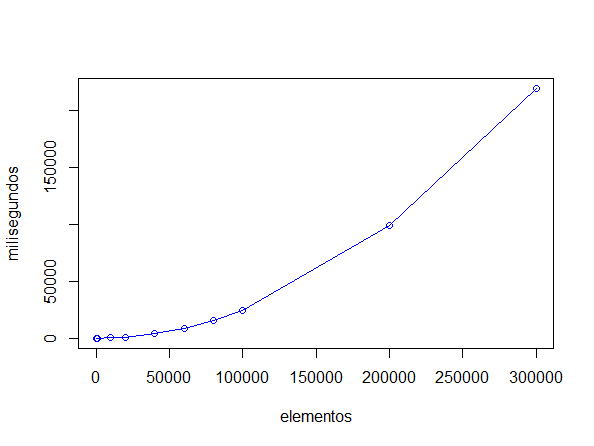
\includegraphics[width=0.8\textwidth]{graph/bubbleSortTime}
\end{center}
\caption{Tiempos en función del número de elementos usando el algoritmo Bubble Short}
\label{fig:bubbleSortTime}
\end{figure}

\subsubsection{Ejemplo en C++}

\showprog{bubbleSortCode.cpp}

\newpage

% ----------------------------------

\subsection{Ordenamiento por selección}

El ordenamiento por selección (Selection Sort en inglés) es un algoritmo de ordenamiento que requiere ${\displaystyle (n^{2})}$ operaciones para ordenar una lista de n elementos.

\subsubsection{Descripción del algoritmo}
Este algoritmo funciona de forma muy intuitiva, en esencia hace lo siguiente:

\begin{itemize}
	\item Buscar el mínimo elemento de la lista
    \item Intercambiarlo con el primero
    \item Buscar el siguiente mínimo en el resto de la lista
    \item Intercambiarlo con el segundo
\end{itemize}
Y en general:
\begin{itemize}
   \item  Buscar el mínimo elemento entre una posición i y el final de la lista
    \item Intercambiar el mínimo con el elemento de la posición i
\end{itemize}

De esta manera se puede escribir el siguiente pseudocódigo para ordenar una lista de n elementos indexados desde el 1:
\begin{quote}
para i=0 hasta n-1\\
    \tab mínimo = i;\\
    \tab para j=i+1 hasta n\\
        \tab \tab si lista[j] < lista[mínimo] entonces\\
            \tab \tab \tab mínimo = j /* (!) */\\
        \tab \tab fin si\\
    \tab fin para\\
    \tab intercambiar(lista[i], lista[mínimo])\\
fin para\\
\end{quote}

Un ejemplo gráfico de este algoritmo se muestra en la figura \ref{fig:selectionSortInfo}.

\begin{figure}[h]
\begin{center}
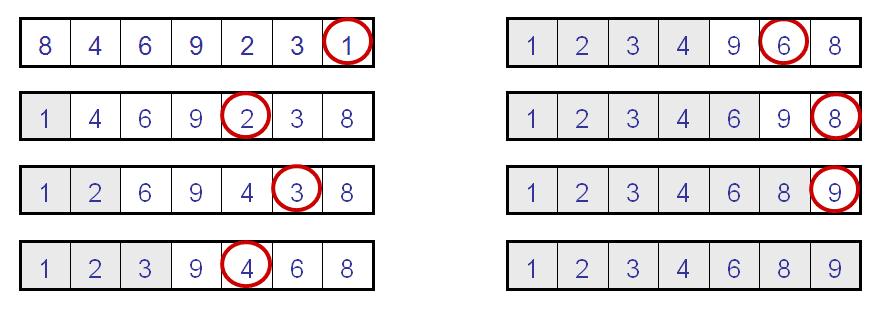
\includegraphics[width=1\textwidth]{graph/selectionSortInfo}
\end{center}
\caption{Ejemplo de funcionamiento del algoritmo de selección}
\label{fig:selectionSortInfo}
\end{figure}

\subsubsection{Análisis}
 
Al algoritmo de ordenamiento por selección, para ordenar un vector de n términos, tiene que realizar siempre el mismo número de comparaciones:

\begin{center}
${\displaystyle c(n)={\frac {n^{2}-n}{2}}}$
\end{center}

Esto es, el número de comparaciones c(n) no depende del orden de los términos, si no del número de términos.

\begin{center}
    ${\displaystyle \Theta (c(n))=n^{2}\;}$
\end{center}

Por lo tanto la cota ajustada asintótica del número de comparaciones pertenece al orden de n cuadrado.

El número de intercambios i(n), también es fijo, téngase en cuenta que la instrucción: \textbf{intercambiar(lista[i], lista[mínimo])} siempre se ejecuta, aun cuando i= mínimo, lo que da lugar:

\begin{center}
    ${\displaystyle i(n)=n\;}$
\end{center}

Sea cual sea el vector, y el orden de sus términos, lo que implica en todos los casos un coste lineal:

\begin{center}
    ${\displaystyle \Theta (i(n))=n\;}$
\end{center}

La cota ajustada asintótica del número de intercambios es lineal, del orden de n.

Asimismo, la fórmula que representa el rendimiento del algoritmo, viene dada por la función:

\begin{center}
    ${\displaystyle c(n)={\frac {n^{2}+n}{2}}}$
\end{center}

\subsubsection{Estudio experimental}
Verificación empírica del análisis, se usará el codigo de ejemplo de la siguiente sección para analizar los tiempos en funcion del tamaño de entrada (eliminando toda funcionalidad de escritura en pantalla para agilizar el proceso y usando los tamaños del algoritmo anterior).

Tras medir los tiempos se deduce experimentalmente (se aprecia en la figura \ref{fig:selectionSortTime}) que el orden de este algoritmo en tiempo es $O(n^2)$, aunque es ligueramente más óptimo que el algoritmo anterior ya que aun siendo un crecimiento exponencial es menor en escala (se dice que su orden exacto es menor, esto se puede apreciar en el apartado de análisis anterior comparándolo con el del algoritmo Bubble Sort).

\begin{figure}[h]
\begin{center}
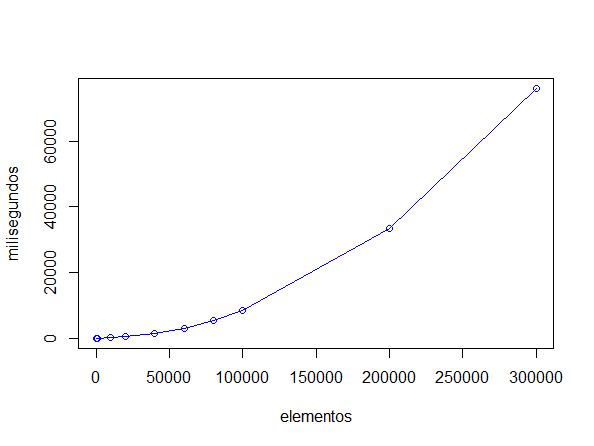
\includegraphics[width=0.5\textwidth]{graph/selectionSortTime}
\end{center}
\caption{Tiempos en función del número de elementos usando el algoritmo SelectionSort}
\label{fig:selectionSortTime}
\end{figure}

\subsubsection{Ejemplo en C++}

\showprog{selectionSort.cpp}

\newpage

% ----------------------------------

\subsection{Ordenamiento Quicksort}
El ordenamiento rápido (quicksort en inglés) es un algoritmo creado por el científico británico en computación C. A. R. Hoare.
El algoritmo trabaja de la siguiente forma (se aprecia en la figura \ref{fig:QuickSortInfo}):

\begin{itemize}
    \item Elegir un elemento de la lista de elementos a ordenar, al que llamaremos pivote.
    \item Resituar los demás elementos de la lista a cada lado del pivote, de manera que a un lado queden todos los menores que él, y al otro los mayores. Los elementos iguales al pivote pueden ser colocados tanto a su derecha como a su izquierda, dependiendo de la implementación deseada. En este momento, el pivote ocupa exactamente el lugar que le corresponderá en la lista ordenada.
    \item La lista queda separada en dos sublistas, una formada por los elementos a la izquierda del pivote, y otra por los elementos a su derecha.
    \item Repetir este proceso de forma recursiva para cada sublista mientras éstas contengan más de un elemento. Una vez terminado este proceso todos los elementos estarán ordenados.
\end{itemize}

\begin{figure}[h]
\begin{center}
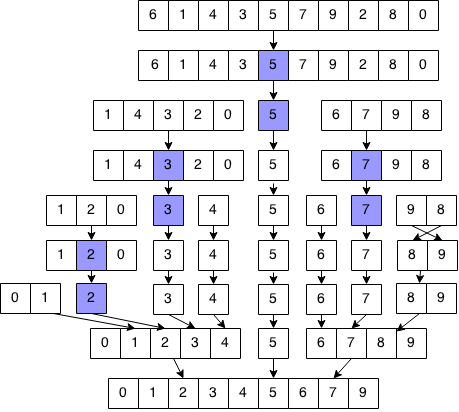
\includegraphics[width=0.5\textwidth]{graph/quick-sort-info}
\end{center}
\caption{Ejemplo de funcionamiento del algoritmo Quick Sort}
\label{fig:QuickSortInfo}
\end{figure}

Como se puede suponer, la eficiencia del algoritmo depende de la posición en la que termine el pivote elegido.

\begin{itemize}
    \item En el mejor caso, el pivote termina en el centro de la lista, dividiéndola en dos sublistas de igual tamaño. En este caso, el orden de complejidad del algoritmo es $O(nlog n)$.
    \item En el peor caso, el pivote termina en un extremo de la lista. El orden de complejidad del algoritmo es entonces de $O(n^2)$. El peor caso dependerá de la implementación del algoritmo, aunque habitualmente ocurre en listas que se encuentran ordenadas, o casi ordenadas. Pero principalmente depende del pivote, si por ejemplo el algoritmo implementado toma como pivote siempre el primer elemento del array, y el array que le pasamos está ordenado, siempre va a generar a su izquierda un array vacío, lo que es ineficiente.

    \item En el caso promedio, el orden es $O(nlog n)$.
\end{itemize}

No es extraño, pues, que la mayoría de optimizaciones que se aplican al algoritmo se centren en la elección del pivote.

\subsubsection{Demostración de un caso particular}
Supongamos que el número de elementos a ordenar es una potencia de dos, es decir, ${\displaystyle n=2^{k}}$ para algún natural ${\displaystyle k}$. Inmediatamente ${\displaystyle k=log_{2}(n)}$, donde k es el número de divisiones que realizará el algoritmo.

En la primera fase del algoritmo habrá n comparaciones. En la segunda fase el algoritmo instanciará dos sublistas de tamaño aproximadamente n/2. El número total de comparaciones de estas dos sublistas es: 2(n/2) = n. En la tercera fase el algoritmo procesará 4 sublistas más, por tanto el número total de comparaciones en esta fase es 4(n/4) = n.

En conclusión, el número total de comparaciones que hace el algoritmo es:

$ {\displaystyle n+n+n+.....+n=kn}$, donde ${\displaystyle k=log_{2}(n)}$, por tanto el Orden de Complejidad del algoritmo en el mejor de los casos es ${\displaystyle O(nlog_{2}(n))}$.

\bigskip

\subsubsection{Técnicas de elección del pivote}
El algoritmo básico del método Quicksort consiste en tomar cualquier elemento de la lista al cual denominaremos como pivote, dependiendo de la partición en que se elija, el algoritmo será más o menos eficiente.
\begin{itemize}
    \item Tomar un elemento cualquiera como pivote tiene la ventaja de no requerir ningún cálculo adicional, lo cual lo hace bastante rápido. Sin embargo, esta elección «a ciegas» siempre provoca que el algoritmo tenga un orden de $O(n^2)$ para ciertas permutaciones de los elementos en la lista.
    \item Otra opción puede ser recorrer la lista para saber de antemano qué elemento ocupará la posición central de la lista, para elegirlo como pivote. Esto puede hacerse en $O(n)$ y asegura que hasta en el peor de los casos, el algoritmo sea $O(n log(n))$. No obstante, el cálculo adicional rebaja bastante la eficiencia del algoritmo en el caso promedio.
    \item La opción a medio camino es tomar tres elementos de la lista - por ejemplo, el primero, el segundo, y el último - y compararlos, eligiendo el valor del medio como pivote.
\end{itemize}

\bigskip

\subsubsection{Técnicas de reposicionamiento}
Una idea preliminar para ubicar el pivote en su posición final sería contar la cantidad de elementos menores que él, y colocarlo un lugar más arriba, moviendo luego todos esos elementos menores que él a su izquierda, para que pueda aplicarse la recursividad.

Existe, no obstante, un procedimiento mucho más efectivo. Se utilizan dos índices: i, al que llamaremos índice izquierdo, y j, al que llamaremos índice derecho. El algoritmo es el siguiente:
\begin{itemize}
    \item Recorrer la lista simultáneamente con i y j: por la izquierda con i (desde el primer elemento), y por la derecha con j (desde el último elemento).
    \item Cuando lista[i] sea mayor que el pivote y lista[j] sea menor, se intercambian los elementos en esas posiciones.
    \item Repetir esto hasta que se crucen los índices.
    \item El punto en que se cruzan los índices es la posición adecuada para colocar el pivote, porque sabemos que a un lado los elementos son todos menores y al otro son todos mayores (o habrían sido intercambiados).
\end{itemize}

\newpage

\subsubsection{Estudio experimental}
Verificación empírica del análisis, se usará el codigo de ejemplo de la siguiente sección para analizar los tiempos en funcion del tamaño de entrada (eliminando toda funcionalidad de escritura en pantalla para agilizar el proceso).

Haciendo uso de una entrada de numeros aleatorios se prueban los casos de 10, 100, 1000, 10000, 20000, 40000, 60000, 80000, 100000, 200000 y 300000 elementos.
Tras medir los tiempos se deduce experimentalmente (se aprecia en la figura \ref{fig:quicksortTime}) que el orden de este algoritmo en tiempo es casi $O(n)$ en este tamaño de problemas, para tamaño mas grandes se apreciara como la grafica tiende a un orden  $O(nlog(n))$.

\begin{figure}[h]
\begin{center}
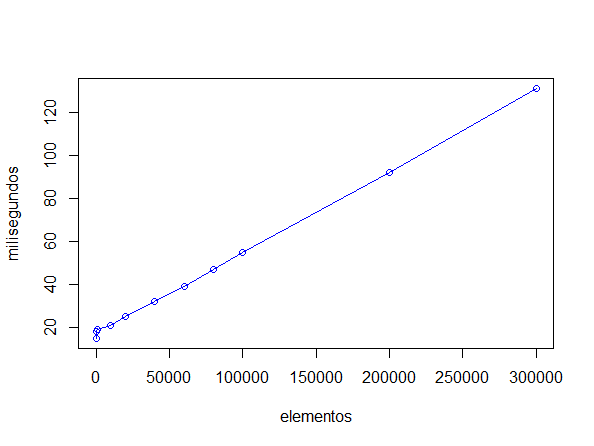
\includegraphics[width=0.8\textwidth]{graph/quicksortTime}
\end{center}
\caption{Tiempos en función del número de elementos usando el algoritmo QuickSort}
\label{fig:quicksortTime}
\end{figure}

\subsubsection{Ejemplo en C++}

\showprog{quicksort.cpp}


\section{Conclusiones}
Se aprecia como el mejor algoritmo de ordenacion es QuickSort, aunque este tiene la limitación de no tener un orden exacto, el promedio como se indica anteriormente es $O(nlog(n))$ pero en el peor caso asciende a un  $O(n^2)$.


\end{document}